% !TEX root =  ../main_manuscript.tex 
\section{Demonstration of Personalized Schedules}
\label{sec:results}
To demonstrate the application of personalized schedules on real patients, we return to the prostate cancer active surveillance dataset, PRIAS, described in Section~\ref{sec:introduction}. The current PRIAS protocol for biopsies is fixed biopsies at year one, four, seven, and ten of follow-up, and every five years after that. Additional annual biopsies are scheduled if a patient's PSA doubling-time~\citep{bokhorst2015compliance} is high. The PSA is measured as per a fixed schedule, quarterly for the first two years, and semi-annually after that. The DRE is also measured semi-annually. The dataset is summarized in Web-Appendix~B.

The clinical data that we intend to use consists of longitudinal PSA (continuous: ng/mL) and DRE (binary: tumor palpable or not) measurements, patient age at baseline, history of biopsies, and interval-censored times of cancer progression. The event of interest is cancer progression. We aim to use the accumulated clinical data to build a joint model that can be utilized for creating personalized biopsy schedules in future PRIAS patients.

\subsection{Fitting the Joint Model to the PRIAS Dataset}
We fit a joint model with $\log_2(\mbox{PSA} + 1)$ transformed PSA~\citep{lin2000latent,pearson1994mixed}, and DRE as longitudinal outcomes, and cancer progression as the event (Web-Appendix~B.3 for exact specification). For PSA, we utilize a linear mixed-effects sub-model wherein PSA profiles are modeled non-linearly over follow-up using B-splines~\citep{de1978practical}. For DRE, we utilize a logistic mixed-effects sub-model. To link the longitudinal sub-models for the PSA and DRE with the relative-risk sub-model for cancer progression, we include three features of the longitudinal outcomes in the relative-risk sub-model. Specifically, the hazard of cancer progression at time $t$ depends on the fitted instantaneous $\log_2(\mbox{PSA} + 1)$ value at time $t$, the estimated instantaneous $\log_2(\mbox{PSA} + 1)$ velocity at $t$, and fitted log-odds of having a DRE indicating a palpable tumor at $t$. We estimated the parameters of our model under the Bayesian framework using the R package \textbf{JMbayes}~\citep{rizopoulosJMbayes}.  

The follow-up period of PRIAS is currently limited. Hence, our joint model is able to predict the cumulative-risk of progression only until the year ten of follow-up. The cumulative-risk of progression at year ten in PRIAS is 50\% (Web-Figure~1). We found that the strongest predictor for progression in our model is $\log_2(\mbox{PSA} + 1)$ velocity. Specifically, for an increase in fitted $\log_2(\mbox{PSA} + 1)$ velocity from -0.03 to 0.15 the adjusted hazard ratio of progression was 1.6 (95\%CI: 1.45--1.78). Detailed parameter estimates are in Web-Appendix~B.4. Since personalized schedules are risk-based, their overall performance is dependent on the predictive accuracy of the fitted model. In this regard, the PRIAS based model's time-dependent area under the receiver operating characteristic curve~\citep{rizopoulos2011dynamic} was moderate (between 0.61 and 0.68) and time-dependent mean absolute prediction error~\citep{rizopoulos2011dynamic} was moderate to large (between 0.08 and 0.24) over follow-up (Web-Appendix~B.6).

\subsection{Personalized Schedules for a Demonstration Patient}
We utilized the joint model fitted to the PRIAS dataset to schedule biopsies in a real PRIAS patient (Figure~\ref{fig:demo_schedule}), starting from his current visit at year five, until year ten of follow-up. This patient has not progressed until year 3.5, and hence even if he incurs a delay in detecting progression of up to three years, it may not lead to adverse outcomes~\citep{carvalho}. Also, since his cumulative-risk of progression at year ten is only 16.5\%, he is likely to progress slowly. Consequently, few biopsies are planned by risk-based personalized schedules (Panel~B, Figure~\ref{fig:demo_schedule}). Even if this patient progresses before year ten of follow-up and opts for personalized schedules, not only will he undergo fewer biopsies than annual schedule (Panel~C, Figure~\ref{fig:demo_schedule}), but his expected delay in detecting progression is also under the aforementioned limit of three years (Panel~D, Figure~\ref{fig:demo_schedule}).
\begin{figure}
\centerline{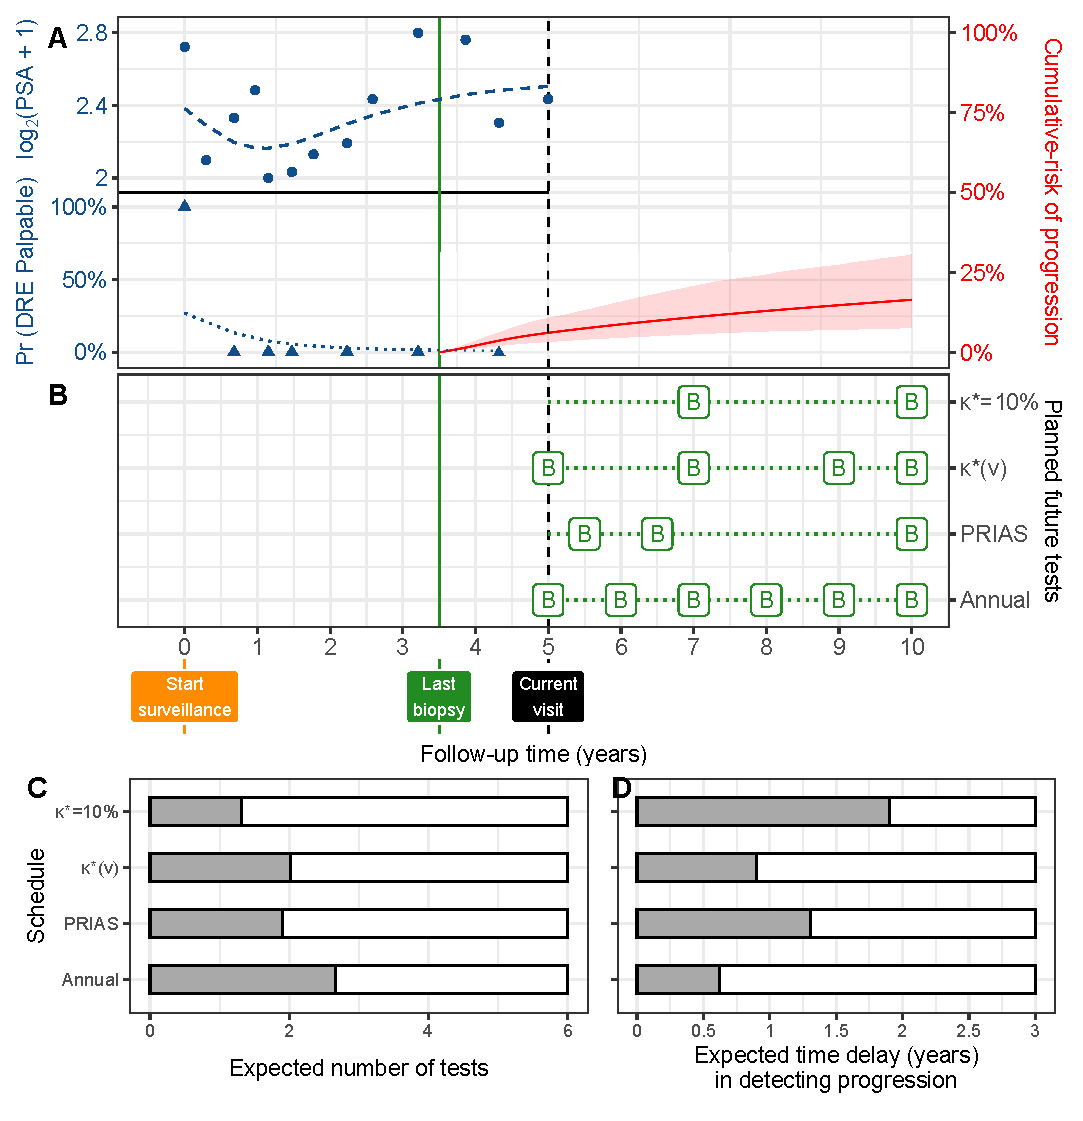
\includegraphics{images/demo_schedule.eps}}
\caption{\textbf{Demonstration of personalized schedules for a real PRIAS patient:} In \textbf{Panel~A}: Time of last negative biopsy is year 3.5 (vertical green solid line). Longitudinal data is repeated DRE (blue triangles) and PSA measurements (blue circles). The current visit is year five (vertical black dashed line). The estimated cumulative-risk profile is shown with a solid red line (95\% credible interval is shaded). It is 16.5\% at year ten (horizon). In \textbf{Panel~B}, we visualize different biopsy schedules, with a `B' indicating a biopsy. \textbf{$\kappa^*=10\%$} and \textbf{$\kappa^*(v)$} are personalized biopsy schedules using a fixed risk threshold of 10\%, and automatically chosen threshold~(\ref{eq:kappa_choice}), respectively. PRIAS and Annual denote the PRIAS biopsy schedule (paragraph~2 of Section~\ref{sec:results}) and annual biopsy schedule. \textbf{Panel~C,D}: For all schedules we calculate the expected number of tests and expected time delay in detecting progression if the patient progresses before year ten. Since a recommended minimum gap of one year is maintained between biopsies, maximum possible number of tests are six.  A delay in detecting progression of up to three years may not lead to adverse outcomes~\citep{carvalho}. }\label{fig:demo_schedule}
\end{figure}